\documentclass[12pt]{article}
\usepackage{blindtext}
\usepackage{geometry}
\usepackage{mathptmx} % Times-New Roman Like
\usepackage{biblatex}

% difffferent style for pandas.styler.to_latex()
\usepackage{booktabs}
\usepackage{multirow}
\usepackage[table]{xcolor}
\usepackage{siunitx}
\usepackage{longtable}
\usepackage{hyperref}

\usepackage{wrapfig} % wrapping 


\usepackage{svg}


\usepackage{pdflscape} % with pdfLatex or LuaLatex
%\usepackage{lscape} % lscape.sty Produce landscape pages in a (mainly) portrait document.
\usepackage{rotating}

%Set the font (output) encoding
%--------------------------------------
\usepackage[T1]{fontenc} %Not needed by LuaLaTeX or XeLaTeX

%French-specific commands
%--------------------------------------
\usepackage[french]{babel}
\usepackage[autolanguage]{numprint} % for the \nombre command

%Hyphenation rules
%--------------------------------------
\usepackage{hyphenat}

\graphicspath{{media/}} % Specifies where to look for included images (trailing slash required)


 \geometry{
letterpaper,
% total={170mm,257mm},
 left=20mm, right=20mm,
 top=20mm, bottom=20mm
 }
 \title{IND6212: Titre du projet}
\author{Ronan Cimadure | Paulo Victor Correia | Chahine Bargaoui  \\ code source: https://github.com/cimadure/ind6212.git}
\date{27 Avril 2023}


%% Set up the bibliography
\addbibresource{report.bib}


\begin{document}
\maketitle

\section{Problématique}
\blindtext[3]
\section{Travaux existants}
\blindtext[1]
\section{Méthodologie}
- source des données \\
Je cite cette source \cite{example-article}\\
\subsection{description des données (taille, format)}

%[!htbp]

\begin{wrapfigure}{r}{0.75\textwidth}
    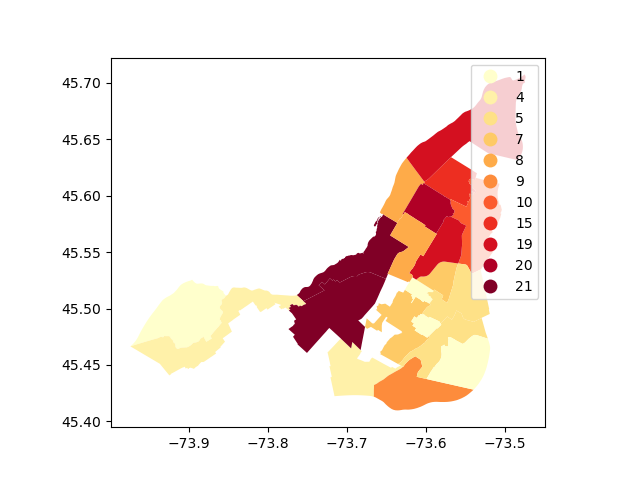
\includegraphics[width=1\linewidth]{media/nombre_de_secteurs_par_arrondissement.png} 
    \caption{Caption1}
    \label{fig:nspa}
\end{wrapfigure}

\subsection{Préparation des données}




- Choix des outils vs problématique  
- Formatage des données vs outil  
- Choix et justification des paramêtres outil  


\begin{wrapfigure}{c}{0.5\textwidth}
    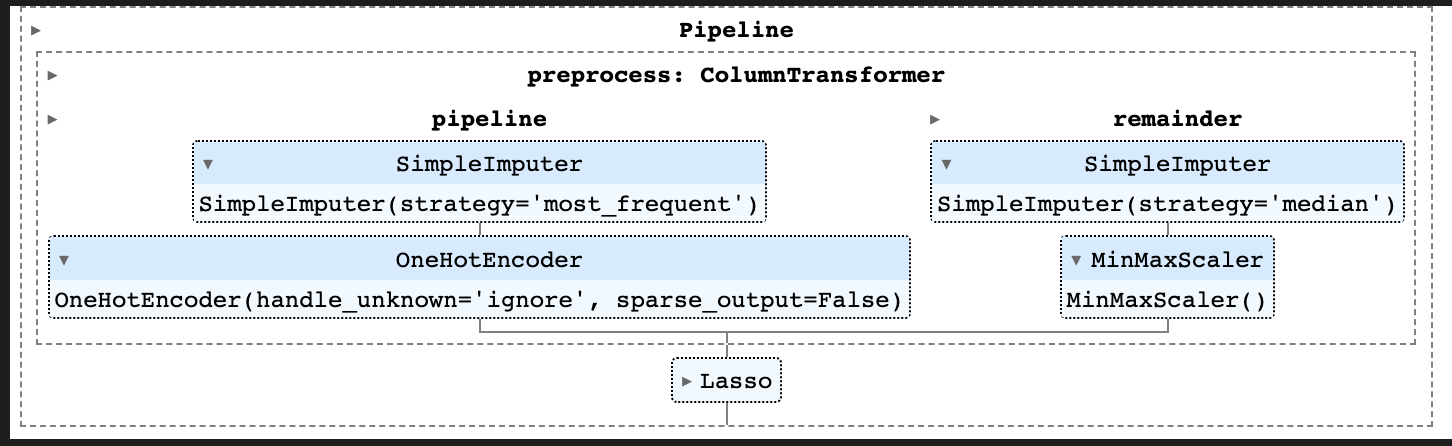
\includegraphics[width=1.0 \linewidth]{media/edited/pipeline.png} 
    \caption{Captijkjon1}
    \label{fig:pipeline}
\end{wrapfigure}

\blindtext[3]



\begin{figure}
    \includesvg[width=1\linewidth]{media/abbreviation_arrondissement.svg} 
    \caption{Caption2}
    \label{fig:arr}
\end{figure}

\begin{wraptable}{l}{10cm}
    \begin{tabular}{lrr}
\toprule
{} &  IdenfiantSecteur &          area \\
ArrondissementCode &                   &               \\
\midrule
AHU                &                21 &  5.214740e+07 \\
SLA                &                21 &  8.764706e+07 \\
SLE                &                20 &  2.759526e+07 \\
RDP                &                19 &  1.049463e+08 \\
RPP                &                19 &  3.239825e+07 \\
ANJ                &                15 &  2.839600e+07 \\
MHM                &                10 &  5.594018e+07 \\
LAS                &                 9 &  5.118610e+07 \\
VSP                &                 8 &  3.361519e+07 \\
MTN                &                 8 &  2.546462e+07 \\
CDN                &                 7 &  4.371704e+07 \\
PMR                &                 7 &  1.659381e+07 \\
VMA                &                 5 &  4.378179e+07 \\
S-O                &                 5 &  3.680719e+07 \\
PRF                &                 4 &  6.913448e+07 \\
LAC                &                 4 &  4.584992e+07 \\
OUT                &                 1 &  7.734627e+06 \\
VER                &                 1 &  4.530048e+07 \\
IBI                &                 1 &  7.391537e+07 \\
WES                &                 1 &  8.175807e+06 \\
\bottomrule
\end{tabular}

    \caption{arr feat 2}
    \label{tab:arrft2}

\end{wraptable}


\begin{landscape}

    \section{Analyse des Resultats}

    \blindtext[6]
    \begin{table}
        \let\center\empty
        \let\endcenter\relax
        \centering
        \resizebox{.6\width}{!}{\begin{tabular}{lrrrrrrrrrrrrrrrrrrrrrrrrrrrrrrrrrrrrrr}
\toprule
{} &      n &      m &     k\_avg &  edge\_length\_total &  edge\_length\_avg &  streets\_per\_node\_avg &  intersection\_count &  street\_length\_total &  street\_segment\_count &  street\_length\_avg &  circuity\_avg &  self\_loop\_proportion &  streets\_per\_node\_counts\_0 &  streets\_per\_node\_counts\_1 &  streets\_per\_node\_counts\_2 &  streets\_per\_node\_counts\_3 &  streets\_per\_node\_counts\_4 &  streets\_per\_node\_counts\_5 &  streets\_per\_node\_proportions\_0 &  streets\_per\_node\_proportions\_1 &  streets\_per\_node\_proportions\_2 &  streets\_per\_node\_proportions\_3 &  streets\_per\_node\_proportions\_4 &  streets\_per\_node\_proportions\_5 &  streets\_per\_node\_counts\_6 &  streets\_per\_node\_proportions\_6 &  streets\_per\_node\_counts\_7 &  streets\_per\_node\_proportions\_7 &  streets\_per\_node\_counts\_8 &  streets\_per\_node\_proportions\_8 &  streets\_per\_node\_counts\_9 &  streets\_per\_node\_proportions\_9 &  streets\_per\_node\_counts\_10 &  streets\_per\_node\_counts\_11 &  streets\_per\_node\_counts\_12 &  streets\_per\_node\_proportions\_10 &  streets\_per\_node\_proportions\_11 &  streets\_per\_node\_proportions\_12 \\
\midrule
AJ &   3119 &   8532 &  5.470984 &         461789.932 &        54.124465 &              3.094902 &                2822 &           277921.879 &                  4776 &          58.191348 &      1.065034 &              0.002513 &                          0 &                        297 &                          9 &                       1930 &                        867 &                       16.0 &                             0.0 &                        0.095223 &                        0.002886 &                        0.618788 &                        0.277974 &                        0.005130 &                        NaN &                             NaN &                        NaN &                             NaN &                        NaN &                             NaN &                        NaN &                             NaN &                         NaN &                         NaN &                         NaN &                              NaN &                              NaN &                              NaN \\
PC &   6325 &  17445 &  5.516206 &         809320.029 &        46.392664 &              2.922213 &                5236 &           439076.017 &                  9180 &          47.829631 &      1.065537 &              0.001961 &                          0 &                       1089 &                         15 &                       3554 &                       1633 &                       34.0 &                             0.0 &                        0.172174 &                        0.002372 &                        0.561897 &                        0.258182 &                        0.005375 &                        NaN &                             NaN &                        NaN &                             NaN &                        NaN &                             NaN &                        NaN &                             NaN &                         NaN &                         NaN &                         NaN &                              NaN &                              NaN &                              NaN \\
RO &   6139 &  17057 &  5.556931 &         865298.849 &        50.729838 &              3.241082 &                5688 &           514283.343 &                  9812 &          52.413712 &      1.039422 &              0.001529 &                          0 &                        451 &                         14 &                       3337 &                       2282 &                       51.0 &                             0.0 &                        0.073465 &                        0.002281 &                        0.543574 &                        0.371722 &                        0.008308 &                        4.0 &                        0.000652 &                        NaN &                             NaN &                        NaN &                             NaN &                        NaN &                             NaN &                         NaN &                         NaN &                         NaN &                              NaN &                              NaN &                              NaN \\
KL &   2822 &   8086 &  5.730687 &         428155.708 &        52.950248 &              3.121899 &                2535 &           237506.274 &                  4378 &          54.249948 &      1.111171 &              0.007081 &                          0 &                        287 &                          7 &                       1623 &                        885 &                       20.0 &                             0.0 &                        0.101701 &                        0.002481 &                        0.575124 &                        0.313607 &                        0.007087 &                        NaN &                             NaN &                        NaN &                             NaN &                        NaN &                             NaN &                        NaN &                             NaN &                         NaN &                         NaN &                         NaN &                              NaN &                              NaN &                              NaN \\
WM &    700 &   1933 &  5.522857 &         138408.943 &        71.603178 &              3.078571 &                 633 &            76323.820 &                  1046 &          72.967323 &      1.043247 &              0.000956 &                          0 &                         67 &                          0 &                        452 &                        173 &                        8.0 &                             0.0 &                        0.095714 &                        0.000000 &                        0.645714 &                        0.247143 &                        0.011429 &                        NaN &                             NaN &                        NaN &                             NaN &                        NaN &                             NaN &                        NaN &                             NaN &                         NaN &                         NaN &                         NaN &                              NaN &                              NaN &                              NaN \\
HS &    453 &   1414 &  6.242826 &          69981.091 &        49.491578 &              3.421634 &                 437 &            38592.347 &                   760 &          50.779404 &      1.045026 &              0.005263 &                          0 &                         16 &                          0 &                        217 &                        217 &                        3.0 &                             0.0 &                        0.035320 &                        0.000000 &                        0.479029 &                        0.479029 &                        0.006623 &                        NaN &                             NaN &                        NaN &                             NaN &                        NaN &                             NaN &                        NaN &                             NaN &                         NaN &                         NaN &                         NaN &                              NaN &                              NaN &                              NaN \\
MH &   6993 &  19688 &  5.630774 &        1056255.121 &        53.649691 &              3.232375 &                6403 &           626557.474 &                 11231 &          55.788218 &      1.044986 &              0.002226 &                          0 &                        590 &                         18 &                       3623 &                       2705 &                       54.0 &                             0.0 &                        0.084370 &                        0.002574 &                        0.518090 &                        0.386815 &                        0.007722 &                        2.0 &                        0.000286 &                        1.0 &                        0.000143 &                        NaN &                             NaN &                        NaN &                             NaN &                         NaN &                         NaN &                         NaN &                              NaN &                              NaN &                              NaN \\
SV &   2385 &   5269 &  4.418449 &         165055.813 &        31.325833 &              2.237736 &                1424 &            83976.263 &                  2656 &          31.617569 &      1.093815 &              0.001883 &                          0 &                        961 &                          0 &                       1320 &                        104 &                        NaN &                             0.0 &                        0.402935 &                        0.000000 &                        0.553459 &                        0.043606 &                             NaN &                        NaN &                             NaN &                        NaN &                             NaN &                        NaN &                             NaN &                        NaN &                             NaN &                         NaN &                         NaN &                         NaN &                              NaN &                              NaN &                              NaN \\
SO &   6375 &  18374 &  5.764392 &         876606.010 &        47.709046 &              3.242510 &                5876 &           513561.389 &                 10220 &          50.250625 &      1.039018 &              0.001174 &                          0 &                        499 &                         17 &                       3373 &                       2423 &                       53.0 &                             0.0 &                        0.078275 &                        0.002667 &                        0.529098 &                        0.380078 &                        0.008314 &                        8.0 &                        0.001255 &                        2.0 &                        0.000314 &                        NaN &                             NaN &                        NaN &                             NaN &                         NaN &                         NaN &                         NaN &                              NaN &                              NaN &                              NaN \\
RP &   3908 &  10807 &  5.530706 &        1091808.435 &       101.027893 &              3.097748 &                3549 &           622297.279 &                  6024 &         103.303001 &      1.088807 &              0.006474 &                          0 &                        359 &                         15 &                       2455 &                       1045 &                       32.0 &                             0.0 &                        0.091863 &                        0.003838 &                        0.628199 &                        0.267400 &                        0.008188 &                        2.0 &                        0.000512 &                        NaN &                             NaN &                        NaN &                             NaN &                        NaN &                             NaN &                         NaN &                         NaN &                         NaN &                              NaN &                              NaN &                              NaN \\
BV &   7008 &  17083 &  4.875285 &         371221.975 &        21.730491 &              2.549087 &                4711 &           200586.538 &                  8902 &          22.532750 &      1.068154 &              0.000899 &                          0 &                       2297 &                          5 &                       3291 &                       1394 &                       18.0 &                             0.0 &                        0.327768 &                        0.000713 &                        0.469606 &                        0.198916 &                        0.002568 &                        3.0 &                        0.000428 &                        NaN &                             NaN &                        NaN &                             NaN &                        NaN &                             NaN &                         NaN &                         NaN &                         NaN &                              NaN &                              NaN &                              NaN \\
PM &   4723 &  13847 &  5.863646 &         555204.230 &        40.095633 &              3.436587 &                4491 &           331721.632 &                  8010 &          41.413437 &      1.018851 &              0.000000 &                          0 &                        232 &                          8 &                       2022 &                       2403 &                       45.0 &                             0.0 &                        0.049121 &                        0.001694 &                        0.428118 &                        0.508787 &                        0.009528 &                       12.0 &                        0.002541 &                        0.0 &                        0.000000 &                        1.0 &                        0.000212 &                        NaN &                             NaN &                         NaN &                         NaN &                         NaN &                              NaN &                              NaN &                              NaN \\
VD &   4612 &  11908 &  5.163920 &         284401.714 &        23.883248 &              2.713356 &                3396 &           156310.038 &                  6257 &          24.981627 &      1.100366 &              0.002557 &                          0 &                       1216 &                         12 &                       2290 &                       1068 &                       24.0 &                             0.0 &                        0.263660 &                        0.002602 &                        0.496531 &                        0.231570 &                        0.005204 &                        2.0 &                        0.000434 &                        NaN &                             NaN &                        NaN &                             NaN &                        NaN &                             NaN &                         NaN &                         NaN &                         NaN &                              NaN &                              NaN &                              NaN \\
DO &   3299 &   9489 &  5.752652 &         590115.871 &        62.189469 &              3.060018 &                2919 &           308370.807 &                  4990 &          61.797757 &      1.113319 &              0.005210 &                          0 &                        380 &                         14 &                       1964 &                        911 &                       29.0 &                             0.0 &                        0.115186 &                        0.004244 &                        0.595332 &                        0.276144 &                        0.008791 &                        1.0 &                        0.000303 &                        NaN &                             NaN &                        NaN &                             NaN &                        NaN &                             NaN &                         NaN &                         NaN &                         NaN &                              NaN &                              NaN &                              NaN \\
ME &    613 &   1525 &  4.975530 &         158781.102 &       104.118755 &              2.903752 &                 508 &            88548.109 &                   861 &         102.843332 &      1.090559 &              0.004646 &                          0 &                        105 &                          1 &                        364 &                        135 &                        7.0 &                             0.0 &                        0.171289 &                        0.001631 &                        0.593801 &                        0.220228 &                        0.011419 &                        1.0 &                        0.001631 &                        NaN &                             NaN &                        NaN &                             NaN &                        NaN &                             NaN &                         NaN &                         NaN &                         NaN &                              NaN &                              NaN &                              NaN \\
BU &   2628 &   6521 &  4.962709 &         250462.268 &        38.408567 &              2.550609 &                1857 &           131750.881 &                  3345 &          39.387408 &      1.068158 &              0.003587 &                          0 &                        771 &                          8 &                       1484 &                        361 &                        4.0 &                             0.0 &                        0.293379 &                        0.003044 &                        0.564688 &                        0.137367 &                        0.001522 &                        NaN &                             NaN &                        NaN &                             NaN &                        NaN &                             NaN &                        NaN &                             NaN &                         NaN &                         NaN &                         NaN &                              NaN &                              NaN &                              NaN \\
LC &   4290 &  12431 &  5.795338 &         659822.923 &        53.078829 &              3.091142 &                3723 &           369451.521 &                  6587 &          56.087980 &      1.051156 &              0.002277 &                          0 &                        567 &                         10 &                       2215 &                       1467 &                       27.0 &                             0.0 &                        0.132168 &                        0.002331 &                        0.516317 &                        0.341958 &                        0.006294 &                        3.0 &                        0.000699 &                        0.0 &                        0.000000 &                        1.0 &                        0.000233 &                        NaN &                             NaN &                         NaN &                         NaN &                         NaN &                              NaN &                              NaN &                              NaN \\
CN &   8994 &  25996 &  5.780743 &        1073182.339 &        41.282595 &              3.213031 &                8095 &           627069.753 &                 14326 &          43.771447 &      1.040575 &              0.002094 &                          0 &                        899 &                         12 &                       4459 &                       3543 &                       67.0 &                             0.0 &                        0.099956 &                        0.001334 &                        0.495775 &                        0.393929 &                        0.007449 &                        9.0 &                        0.001001 &                        4.0 &                        0.000445 &                        0.0 &                        0.000000 &                        1.0 &                        0.000111 &                         NaN &                         NaN &                         NaN &                              NaN &                              NaN &                              NaN \\
VS &   7467 &  21051 &  5.638409 &         833283.418 &        39.584030 &              3.196866 &                6592 &           505561.769 &                 11781 &          42.913315 &      1.024785 &              0.000849 &                          0 &                        875 &                         13 &                       3408 &                       3117 &                       46.0 &                             0.0 &                        0.117182 &                        0.001741 &                        0.456408 &                        0.417437 &                        0.006160 &                        8.0 &                        0.001071 &                        NaN &                             NaN &                        NaN &                             NaN &                        NaN &                             NaN &                         NaN &                         NaN &                         NaN &                              NaN &                              NaN &                              NaN \\
ID &    152 &    314 &  4.131579 &           8197.052 &        26.105261 &              2.072368 &                  80 &             4098.526 &                   157 &          26.105261 &      1.030560 &              0.000000 &                          0 &                         72 &                          0 &                         77 &                          3 &                        NaN &                             0.0 &                        0.473684 &                        0.000000 &                        0.506579 &                        0.019737 &                             NaN &                        NaN &                             NaN &                        NaN &                             NaN &                        NaN &                             NaN &                        NaN &                             NaN &                         NaN &                         NaN &                         NaN &                              NaN &                              NaN &                              NaN \\
CL &   1273 &   3589 &  5.638649 &         211707.344 &        58.987836 &              3.185389 &                1152 &           115799.313 &                  1986 &          58.307811 &      1.094430 &              0.004028 &                          0 &                        121 &                          5 &                        672 &                        467 &                        8.0 &                             0.0 &                        0.095051 &                        0.003928 &                        0.527887 &                        0.366850 &                        0.006284 &                        NaN &                             NaN &                        NaN &                             NaN &                        NaN &                             NaN &                        NaN &                             NaN &                         NaN &                         NaN &                         NaN &                              NaN &                              NaN &                              NaN \\
BF &   2151 &   6084 &  5.656904 &         383041.262 &        62.958787 &              2.925151 &                1805 &           202002.629 &                  3132 &          64.496369 &      1.103389 &              0.006386 &                          0 &                        346 &                          0 &                       1282 &                        515 &                        8.0 &                             0.0 &                        0.160855 &                        0.000000 &                        0.596002 &                        0.239424 &                        0.003719 &                        NaN &                             NaN &                        NaN &                             NaN &                        NaN &                             NaN &                        NaN &                             NaN &                         NaN &                         NaN &                         NaN &                              NaN &                              NaN &                              NaN \\
PR &   6189 &  17981 &  5.810632 &         937093.541 &        52.115763 &              3.028276 &                5297 &           480535.188 &                  9291 &          51.720502 &      1.091434 &              0.006243 &                          0 &                        892 &                          9 &                       3370 &                       1875 &                       36.0 &                             0.0 &                        0.144127 &                        0.001454 &                        0.544514 &                        0.302957 &                        0.005817 &                        7.0 &                        0.001131 &                        NaN &                             NaN &                        NaN &                             NaN &                        NaN &                             NaN &                         NaN &                         NaN &                         NaN &                              NaN &                              NaN &                              NaN \\
MN &   1417 &   3699 &  5.220889 &         303884.713 &        82.153207 &              3.310515 &                1372 &           210568.370 &                  2326 &          90.528104 &      1.033541 &              0.005159 &                          0 &                         45 &                          2 &                        850 &                        509 &                       10.0 &                             0.0 &                        0.031757 &                        0.001411 &                        0.599859 &                        0.359210 &                        0.007057 &                        1.0 &                        0.000706 &                        NaN &                             NaN &                        NaN &                             NaN &                        NaN &                             NaN &                         NaN &                         NaN &                         NaN &                              NaN &                              NaN &                              NaN \\
MR &   1454 &   4041 &  5.558459 &         257056.624 &        63.612132 &              3.160935 &                1324 &           143205.943 &                  2238 &          63.988357 &      1.051537 &              0.000894 &                          0 &                        130 &                          6 &                        842 &                        454 &                       20.0 &                             0.0 &                        0.089409 &                        0.004127 &                        0.579092 &                        0.312242 &                        0.013755 &                        2.0 &                        0.001376 &                        NaN &                             NaN &                        NaN &                             NaN &                        NaN &                             NaN &                         NaN &                         NaN &                         NaN &                              NaN &                              NaN &                              NaN \\
MO &    755 &   2326 &  6.161589 &          75959.283 &        32.656613 &              3.225166 &                 666 &            40029.408 &                  1198 &          33.413529 &      1.032076 &              0.001669 &                          0 &                         89 &                          2 &                        316 &                        346 &                        2.0 &                             0.0 &                        0.117881 &                        0.002649 &                        0.418543 &                        0.458278 &                        0.002649 &                        NaN &                             NaN &                        NaN &                             NaN &                        NaN &                             NaN &                        NaN &                             NaN &                         NaN &                         NaN &                         NaN &                              NaN &                              NaN &                              NaN \\
AC &  15016 &  43158 &  5.748269 &        1433695.821 &        33.219700 &              3.121404 &               12872 &           818807.168 &                 23342 &          35.078707 &      1.045131 &              0.001671 &                          0 &                       2144 &                         43 &                       6808 &                       5899 &                      115.0 &                             0.0 &                        0.142781 &                        0.002864 &                        0.453383 &                        0.392848 &                        0.007658 &                        4.0 &                        0.000266 &                        2.0 &                        0.000133 &                        1.0 &                        0.000067 &                        NaN &                             NaN &                         NaN &                         NaN &                         NaN &                              NaN &                              NaN &                              NaN \\
LN &   2731 &   7772 &  5.691688 &         496774.782 &        63.918526 &              3.151227 &                2550 &           276408.153 &                  4257 &          64.930268 &      1.071116 &              0.001175 &                          0 &                        181 &                          6 &                       1782 &                        743 &                       19.0 &                             0.0 &                        0.066276 &                        0.002197 &                        0.652508 &                        0.272062 &                        0.006957 &                        NaN &                             NaN &                        NaN &                             NaN &                        NaN &                             NaN &                        NaN &                             NaN &                         NaN &                         NaN &                         NaN &                              NaN &                              NaN &                              NaN \\
OM &   1191 &   3353 &  5.630563 &         170938.573 &        50.980785 &              3.147775 &                1076 &            94837.159 &                  1838 &          51.598019 &      1.050006 &              0.000544 &                          0 &                        115 &                          3 &                        687 &                        364 &                       21.0 &                             0.0 &                        0.096558 &                        0.002519 &                        0.576826 &                        0.305626 &                        0.017632 &                        1.0 &                        0.000840 &                        NaN &                             NaN &                        NaN &                             NaN &                        NaN &                             NaN &                         NaN &                         NaN &                         NaN &                              NaN &                              NaN &                              NaN \\
VM &   8509 &  23656 &  5.560230 &         998454.564 &        42.207244 &              3.202256 &                7683 &           581872.130 &                 13481 &          43.162386 &      1.046780 &              0.001780 &                          0 &                        826 &                         34 &                       4355 &                       3193 &                       92.0 &                             0.0 &                        0.097074 &                        0.003996 &                        0.511811 &                        0.375250 &                        0.010812 &                        7.0 &                        0.000823 &                        1.0 &                        0.000118 &                        1.0 &                        0.000118 &                        NaN &                             NaN &                         NaN &                         NaN &                         NaN &                              NaN &                              NaN &                              NaN \\
IS &   2180 &   6072 &  5.570642 &         425913.761 &        70.143900 &              2.844495 &                1769 &           214662.661 &                  3078 &          69.740955 &      1.214817 &              0.011371 &                          0 &                        411 &                          2 &                       1293 &                        463 &                       11.0 &                             0.0 &                        0.188532 &                        0.000917 &                        0.593119 &                        0.212385 &                        0.005046 &                        NaN &                             NaN &                        NaN &                             NaN &                        NaN &                             NaN &                        NaN &                             NaN &                         NaN &                         NaN &                         NaN &                              NaN &                              NaN &                              NaN \\
DV &   4179 &  11324 &  5.419478 &         616064.121 &        54.403402 &              2.959320 &                3545 &           345153.495 &                  6144 &          56.177327 &      1.084796 &              0.003092 &                          0 &                        634 &                         13 &                       2452 &                       1058 &                       19.0 &                             0.0 &                        0.151711 &                        0.003111 &                        0.586743 &                        0.253171 &                        0.004547 &                        2.0 &                        0.000479 &                        0.0 &                        0.000000 &                        0.0 &                        0.000000 &                        0.0 &                        0.000000 &                         0.0 &                         0.0 &                         1.0 &                              0.0 &                              0.0 &                         0.000239 \\
LR &  13213 &  37162 &  5.625066 &        1825126.158 &        49.112700 &              3.110724 &               11718 &          1038519.517 &                 20443 &          50.800739 &      1.067572 &              0.002641 &                          0 &                       1495 &                         28 &                       7321 &                       4268 &                       93.0 &                             0.0 &                        0.113146 &                        0.002119 &                        0.554076 &                        0.323015 &                        0.007039 &                        6.0 &                        0.000454 &                        1.0 &                        0.000076 &                        1.0 &                        0.000076 &                        NaN &                             NaN &                         NaN &                         NaN &                         NaN &                              NaN &                              NaN &                              NaN \\
LS &   6869 &  20422 &  5.946135 &         887590.024 &        43.462444 &              3.158830 &                6129 &           477262.302 &                 10833 &          44.056337 &      1.052926 &              0.001015 &                          0 &                        740 &                         21 &                       3558 &                       2515 &                       28.0 &                             0.0 &                        0.107730 &                        0.003057 &                        0.517979 &                        0.366138 &                        0.004076 &                        7.0 &                        0.001019 &                        NaN &                             NaN &                        NaN &                             NaN &                        NaN &                             NaN &                         NaN &                         NaN &                         NaN &                              NaN &                              NaN &                              NaN \\
\bottomrule
\end{tabular}
}
    \end{table} 

    \begin{wraptable}{l}{1.0\textwidth}
        \begin{tabular}{lrrrrrrrrrrrrrrrrrrrrrrrrrrrrrrrrrrrrrr}
\toprule
{} &      n &      m &     k\_avg &  edge\_length\_total &  edge\_length\_avg &  streets\_per\_node\_avg &  intersection\_count &  street\_length\_total &  street\_segment\_count &  street\_length\_avg &  circuity\_avg &  self\_loop\_proportion &  streets\_per\_node\_counts\_0 &  streets\_per\_node\_counts\_1 &  streets\_per\_node\_counts\_2 &  streets\_per\_node\_counts\_3 &  streets\_per\_node\_counts\_4 &  streets\_per\_node\_counts\_5 &  streets\_per\_node\_proportions\_0 &  streets\_per\_node\_proportions\_1 &  streets\_per\_node\_proportions\_2 &  streets\_per\_node\_proportions\_3 &  streets\_per\_node\_proportions\_4 &  streets\_per\_node\_proportions\_5 &  streets\_per\_node\_counts\_6 &  streets\_per\_node\_proportions\_6 &  streets\_per\_node\_counts\_7 &  streets\_per\_node\_proportions\_7 &  streets\_per\_node\_counts\_8 &  streets\_per\_node\_proportions\_8 &  streets\_per\_node\_counts\_9 &  streets\_per\_node\_proportions\_9 &  streets\_per\_node\_counts\_10 &  streets\_per\_node\_counts\_11 &  streets\_per\_node\_counts\_12 &  streets\_per\_node\_proportions\_10 &  streets\_per\_node\_proportions\_11 &  streets\_per\_node\_proportions\_12 \\
\midrule
AJ &   3119 &   8532 &  5.470984 &         461789.932 &        54.124465 &              3.094902 &                2822 &           277921.879 &                  4776 &          58.191348 &      1.065034 &              0.002513 &                          0 &                        297 &                          9 &                       1930 &                        867 &                       16.0 &                             0.0 &                        0.095223 &                        0.002886 &                        0.618788 &                        0.277974 &                        0.005130 &                        NaN &                             NaN &                        NaN &                             NaN &                        NaN &                             NaN &                        NaN &                             NaN &                         NaN &                         NaN &                         NaN &                              NaN &                              NaN &                              NaN \\
PC &   6325 &  17445 &  5.516206 &         809320.029 &        46.392664 &              2.922213 &                5236 &           439076.017 &                  9180 &          47.829631 &      1.065537 &              0.001961 &                          0 &                       1089 &                         15 &                       3554 &                       1633 &                       34.0 &                             0.0 &                        0.172174 &                        0.002372 &                        0.561897 &                        0.258182 &                        0.005375 &                        NaN &                             NaN &                        NaN &                             NaN &                        NaN &                             NaN &                        NaN &                             NaN &                         NaN &                         NaN &                         NaN &                              NaN &                              NaN &                              NaN \\
RO &   6139 &  17057 &  5.556931 &         865298.849 &        50.729838 &              3.241082 &                5688 &           514283.343 &                  9812 &          52.413712 &      1.039422 &              0.001529 &                          0 &                        451 &                         14 &                       3337 &                       2282 &                       51.0 &                             0.0 &                        0.073465 &                        0.002281 &                        0.543574 &                        0.371722 &                        0.008308 &                        4.0 &                        0.000652 &                        NaN &                             NaN &                        NaN &                             NaN &                        NaN &                             NaN &                         NaN &                         NaN &                         NaN &                              NaN &                              NaN &                              NaN \\
KL &   2822 &   8086 &  5.730687 &         428155.708 &        52.950248 &              3.121899 &                2535 &           237506.274 &                  4378 &          54.249948 &      1.111171 &              0.007081 &                          0 &                        287 &                          7 &                       1623 &                        885 &                       20.0 &                             0.0 &                        0.101701 &                        0.002481 &                        0.575124 &                        0.313607 &                        0.007087 &                        NaN &                             NaN &                        NaN &                             NaN &                        NaN &                             NaN &                        NaN &                             NaN &                         NaN &                         NaN &                         NaN &                              NaN &                              NaN &                              NaN \\
WM &    700 &   1933 &  5.522857 &         138408.943 &        71.603178 &              3.078571 &                 633 &            76323.820 &                  1046 &          72.967323 &      1.043247 &              0.000956 &                          0 &                         67 &                          0 &                        452 &                        173 &                        8.0 &                             0.0 &                        0.095714 &                        0.000000 &                        0.645714 &                        0.247143 &                        0.011429 &                        NaN &                             NaN &                        NaN &                             NaN &                        NaN &                             NaN &                        NaN &                             NaN &                         NaN &                         NaN &                         NaN &                              NaN &                              NaN &                              NaN \\
HS &    453 &   1414 &  6.242826 &          69981.091 &        49.491578 &              3.421634 &                 437 &            38592.347 &                   760 &          50.779404 &      1.045026 &              0.005263 &                          0 &                         16 &                          0 &                        217 &                        217 &                        3.0 &                             0.0 &                        0.035320 &                        0.000000 &                        0.479029 &                        0.479029 &                        0.006623 &                        NaN &                             NaN &                        NaN &                             NaN &                        NaN &                             NaN &                        NaN &                             NaN &                         NaN &                         NaN &                         NaN &                              NaN &                              NaN &                              NaN \\
MH &   6993 &  19688 &  5.630774 &        1056255.121 &        53.649691 &              3.232375 &                6403 &           626557.474 &                 11231 &          55.788218 &      1.044986 &              0.002226 &                          0 &                        590 &                         18 &                       3623 &                       2705 &                       54.0 &                             0.0 &                        0.084370 &                        0.002574 &                        0.518090 &                        0.386815 &                        0.007722 &                        2.0 &                        0.000286 &                        1.0 &                        0.000143 &                        NaN &                             NaN &                        NaN &                             NaN &                         NaN &                         NaN &                         NaN &                              NaN &                              NaN &                              NaN \\
SV &   2385 &   5269 &  4.418449 &         165055.813 &        31.325833 &              2.237736 &                1424 &            83976.263 &                  2656 &          31.617569 &      1.093815 &              0.001883 &                          0 &                        961 &                          0 &                       1320 &                        104 &                        NaN &                             0.0 &                        0.402935 &                        0.000000 &                        0.553459 &                        0.043606 &                             NaN &                        NaN &                             NaN &                        NaN &                             NaN &                        NaN &                             NaN &                        NaN &                             NaN &                         NaN &                         NaN &                         NaN &                              NaN &                              NaN &                              NaN \\
SO &   6375 &  18374 &  5.764392 &         876606.010 &        47.709046 &              3.242510 &                5876 &           513561.389 &                 10220 &          50.250625 &      1.039018 &              0.001174 &                          0 &                        499 &                         17 &                       3373 &                       2423 &                       53.0 &                             0.0 &                        0.078275 &                        0.002667 &                        0.529098 &                        0.380078 &                        0.008314 &                        8.0 &                        0.001255 &                        2.0 &                        0.000314 &                        NaN &                             NaN &                        NaN &                             NaN &                         NaN &                         NaN &                         NaN &                              NaN &                              NaN &                              NaN \\
RP &   3908 &  10807 &  5.530706 &        1091808.435 &       101.027893 &              3.097748 &                3549 &           622297.279 &                  6024 &         103.303001 &      1.088807 &              0.006474 &                          0 &                        359 &                         15 &                       2455 &                       1045 &                       32.0 &                             0.0 &                        0.091863 &                        0.003838 &                        0.628199 &                        0.267400 &                        0.008188 &                        2.0 &                        0.000512 &                        NaN &                             NaN &                        NaN &                             NaN &                        NaN &                             NaN &                         NaN &                         NaN &                         NaN &                              NaN &                              NaN &                              NaN \\
BV &   7008 &  17083 &  4.875285 &         371221.975 &        21.730491 &              2.549087 &                4711 &           200586.538 &                  8902 &          22.532750 &      1.068154 &              0.000899 &                          0 &                       2297 &                          5 &                       3291 &                       1394 &                       18.0 &                             0.0 &                        0.327768 &                        0.000713 &                        0.469606 &                        0.198916 &                        0.002568 &                        3.0 &                        0.000428 &                        NaN &                             NaN &                        NaN &                             NaN &                        NaN &                             NaN &                         NaN &                         NaN &                         NaN &                              NaN &                              NaN &                              NaN \\
PM &   4723 &  13847 &  5.863646 &         555204.230 &        40.095633 &              3.436587 &                4491 &           331721.632 &                  8010 &          41.413437 &      1.018851 &              0.000000 &                          0 &                        232 &                          8 &                       2022 &                       2403 &                       45.0 &                             0.0 &                        0.049121 &                        0.001694 &                        0.428118 &                        0.508787 &                        0.009528 &                       12.0 &                        0.002541 &                        0.0 &                        0.000000 &                        1.0 &                        0.000212 &                        NaN &                             NaN &                         NaN &                         NaN &                         NaN &                              NaN &                              NaN &                              NaN \\
VD &   4612 &  11908 &  5.163920 &         284401.714 &        23.883248 &              2.713356 &                3396 &           156310.038 &                  6257 &          24.981627 &      1.100366 &              0.002557 &                          0 &                       1216 &                         12 &                       2290 &                       1068 &                       24.0 &                             0.0 &                        0.263660 &                        0.002602 &                        0.496531 &                        0.231570 &                        0.005204 &                        2.0 &                        0.000434 &                        NaN &                             NaN &                        NaN &                             NaN &                        NaN &                             NaN &                         NaN &                         NaN &                         NaN &                              NaN &                              NaN &                              NaN \\
DO &   3299 &   9489 &  5.752652 &         590115.871 &        62.189469 &              3.060018 &                2919 &           308370.807 &                  4990 &          61.797757 &      1.113319 &              0.005210 &                          0 &                        380 &                         14 &                       1964 &                        911 &                       29.0 &                             0.0 &                        0.115186 &                        0.004244 &                        0.595332 &                        0.276144 &                        0.008791 &                        1.0 &                        0.000303 &                        NaN &                             NaN &                        NaN &                             NaN &                        NaN &                             NaN &                         NaN &                         NaN &                         NaN &                              NaN &                              NaN &                              NaN \\
ME &    613 &   1525 &  4.975530 &         158781.102 &       104.118755 &              2.903752 &                 508 &            88548.109 &                   861 &         102.843332 &      1.090559 &              0.004646 &                          0 &                        105 &                          1 &                        364 &                        135 &                        7.0 &                             0.0 &                        0.171289 &                        0.001631 &                        0.593801 &                        0.220228 &                        0.011419 &                        1.0 &                        0.001631 &                        NaN &                             NaN &                        NaN &                             NaN &                        NaN &                             NaN &                         NaN &                         NaN &                         NaN &                              NaN &                              NaN &                              NaN \\
BU &   2628 &   6521 &  4.962709 &         250462.268 &        38.408567 &              2.550609 &                1857 &           131750.881 &                  3345 &          39.387408 &      1.068158 &              0.003587 &                          0 &                        771 &                          8 &                       1484 &                        361 &                        4.0 &                             0.0 &                        0.293379 &                        0.003044 &                        0.564688 &                        0.137367 &                        0.001522 &                        NaN &                             NaN &                        NaN &                             NaN &                        NaN &                             NaN &                        NaN &                             NaN &                         NaN &                         NaN &                         NaN &                              NaN &                              NaN &                              NaN \\
LC &   4290 &  12431 &  5.795338 &         659822.923 &        53.078829 &              3.091142 &                3723 &           369451.521 &                  6587 &          56.087980 &      1.051156 &              0.002277 &                          0 &                        567 &                         10 &                       2215 &                       1467 &                       27.0 &                             0.0 &                        0.132168 &                        0.002331 &                        0.516317 &                        0.341958 &                        0.006294 &                        3.0 &                        0.000699 &                        0.0 &                        0.000000 &                        1.0 &                        0.000233 &                        NaN &                             NaN &                         NaN &                         NaN &                         NaN &                              NaN &                              NaN &                              NaN \\
CN &   8994 &  25996 &  5.780743 &        1073182.339 &        41.282595 &              3.213031 &                8095 &           627069.753 &                 14326 &          43.771447 &      1.040575 &              0.002094 &                          0 &                        899 &                         12 &                       4459 &                       3543 &                       67.0 &                             0.0 &                        0.099956 &                        0.001334 &                        0.495775 &                        0.393929 &                        0.007449 &                        9.0 &                        0.001001 &                        4.0 &                        0.000445 &                        0.0 &                        0.000000 &                        1.0 &                        0.000111 &                         NaN &                         NaN &                         NaN &                              NaN &                              NaN &                              NaN \\
VS &   7467 &  21051 &  5.638409 &         833283.418 &        39.584030 &              3.196866 &                6592 &           505561.769 &                 11781 &          42.913315 &      1.024785 &              0.000849 &                          0 &                        875 &                         13 &                       3408 &                       3117 &                       46.0 &                             0.0 &                        0.117182 &                        0.001741 &                        0.456408 &                        0.417437 &                        0.006160 &                        8.0 &                        0.001071 &                        NaN &                             NaN &                        NaN &                             NaN &                        NaN &                             NaN &                         NaN &                         NaN &                         NaN &                              NaN &                              NaN &                              NaN \\
ID &    152 &    314 &  4.131579 &           8197.052 &        26.105261 &              2.072368 &                  80 &             4098.526 &                   157 &          26.105261 &      1.030560 &              0.000000 &                          0 &                         72 &                          0 &                         77 &                          3 &                        NaN &                             0.0 &                        0.473684 &                        0.000000 &                        0.506579 &                        0.019737 &                             NaN &                        NaN &                             NaN &                        NaN &                             NaN &                        NaN &                             NaN &                        NaN &                             NaN &                         NaN &                         NaN &                         NaN &                              NaN &                              NaN &                              NaN \\
CL &   1273 &   3589 &  5.638649 &         211707.344 &        58.987836 &              3.185389 &                1152 &           115799.313 &                  1986 &          58.307811 &      1.094430 &              0.004028 &                          0 &                        121 &                          5 &                        672 &                        467 &                        8.0 &                             0.0 &                        0.095051 &                        0.003928 &                        0.527887 &                        0.366850 &                        0.006284 &                        NaN &                             NaN &                        NaN &                             NaN &                        NaN &                             NaN &                        NaN &                             NaN &                         NaN &                         NaN &                         NaN &                              NaN &                              NaN &                              NaN \\
BF &   2151 &   6084 &  5.656904 &         383041.262 &        62.958787 &              2.925151 &                1805 &           202002.629 &                  3132 &          64.496369 &      1.103389 &              0.006386 &                          0 &                        346 &                          0 &                       1282 &                        515 &                        8.0 &                             0.0 &                        0.160855 &                        0.000000 &                        0.596002 &                        0.239424 &                        0.003719 &                        NaN &                             NaN &                        NaN &                             NaN &                        NaN &                             NaN &                        NaN &                             NaN &                         NaN &                         NaN &                         NaN &                              NaN &                              NaN &                              NaN \\
PR &   6189 &  17981 &  5.810632 &         937093.541 &        52.115763 &              3.028276 &                5297 &           480535.188 &                  9291 &          51.720502 &      1.091434 &              0.006243 &                          0 &                        892 &                          9 &                       3370 &                       1875 &                       36.0 &                             0.0 &                        0.144127 &                        0.001454 &                        0.544514 &                        0.302957 &                        0.005817 &                        7.0 &                        0.001131 &                        NaN &                             NaN &                        NaN &                             NaN &                        NaN &                             NaN &                         NaN &                         NaN &                         NaN &                              NaN &                              NaN &                              NaN \\
MN &   1417 &   3699 &  5.220889 &         303884.713 &        82.153207 &              3.310515 &                1372 &           210568.370 &                  2326 &          90.528104 &      1.033541 &              0.005159 &                          0 &                         45 &                          2 &                        850 &                        509 &                       10.0 &                             0.0 &                        0.031757 &                        0.001411 &                        0.599859 &                        0.359210 &                        0.007057 &                        1.0 &                        0.000706 &                        NaN &                             NaN &                        NaN &                             NaN &                        NaN &                             NaN &                         NaN &                         NaN &                         NaN &                              NaN &                              NaN &                              NaN \\
MR &   1454 &   4041 &  5.558459 &         257056.624 &        63.612132 &              3.160935 &                1324 &           143205.943 &                  2238 &          63.988357 &      1.051537 &              0.000894 &                          0 &                        130 &                          6 &                        842 &                        454 &                       20.0 &                             0.0 &                        0.089409 &                        0.004127 &                        0.579092 &                        0.312242 &                        0.013755 &                        2.0 &                        0.001376 &                        NaN &                             NaN &                        NaN &                             NaN &                        NaN &                             NaN &                         NaN &                         NaN &                         NaN &                              NaN &                              NaN &                              NaN \\
MO &    755 &   2326 &  6.161589 &          75959.283 &        32.656613 &              3.225166 &                 666 &            40029.408 &                  1198 &          33.413529 &      1.032076 &              0.001669 &                          0 &                         89 &                          2 &                        316 &                        346 &                        2.0 &                             0.0 &                        0.117881 &                        0.002649 &                        0.418543 &                        0.458278 &                        0.002649 &                        NaN &                             NaN &                        NaN &                             NaN &                        NaN &                             NaN &                        NaN &                             NaN &                         NaN &                         NaN &                         NaN &                              NaN &                              NaN &                              NaN \\
AC &  15016 &  43158 &  5.748269 &        1433695.821 &        33.219700 &              3.121404 &               12872 &           818807.168 &                 23342 &          35.078707 &      1.045131 &              0.001671 &                          0 &                       2144 &                         43 &                       6808 &                       5899 &                      115.0 &                             0.0 &                        0.142781 &                        0.002864 &                        0.453383 &                        0.392848 &                        0.007658 &                        4.0 &                        0.000266 &                        2.0 &                        0.000133 &                        1.0 &                        0.000067 &                        NaN &                             NaN &                         NaN &                         NaN &                         NaN &                              NaN &                              NaN &                              NaN \\
LN &   2731 &   7772 &  5.691688 &         496774.782 &        63.918526 &              3.151227 &                2550 &           276408.153 &                  4257 &          64.930268 &      1.071116 &              0.001175 &                          0 &                        181 &                          6 &                       1782 &                        743 &                       19.0 &                             0.0 &                        0.066276 &                        0.002197 &                        0.652508 &                        0.272062 &                        0.006957 &                        NaN &                             NaN &                        NaN &                             NaN &                        NaN &                             NaN &                        NaN &                             NaN &                         NaN &                         NaN &                         NaN &                              NaN &                              NaN &                              NaN \\
OM &   1191 &   3353 &  5.630563 &         170938.573 &        50.980785 &              3.147775 &                1076 &            94837.159 &                  1838 &          51.598019 &      1.050006 &              0.000544 &                          0 &                        115 &                          3 &                        687 &                        364 &                       21.0 &                             0.0 &                        0.096558 &                        0.002519 &                        0.576826 &                        0.305626 &                        0.017632 &                        1.0 &                        0.000840 &                        NaN &                             NaN &                        NaN &                             NaN &                        NaN &                             NaN &                         NaN &                         NaN &                         NaN &                              NaN &                              NaN &                              NaN \\
VM &   8509 &  23656 &  5.560230 &         998454.564 &        42.207244 &              3.202256 &                7683 &           581872.130 &                 13481 &          43.162386 &      1.046780 &              0.001780 &                          0 &                        826 &                         34 &                       4355 &                       3193 &                       92.0 &                             0.0 &                        0.097074 &                        0.003996 &                        0.511811 &                        0.375250 &                        0.010812 &                        7.0 &                        0.000823 &                        1.0 &                        0.000118 &                        1.0 &                        0.000118 &                        NaN &                             NaN &                         NaN &                         NaN &                         NaN &                              NaN &                              NaN &                              NaN \\
IS &   2180 &   6072 &  5.570642 &         425913.761 &        70.143900 &              2.844495 &                1769 &           214662.661 &                  3078 &          69.740955 &      1.214817 &              0.011371 &                          0 &                        411 &                          2 &                       1293 &                        463 &                       11.0 &                             0.0 &                        0.188532 &                        0.000917 &                        0.593119 &                        0.212385 &                        0.005046 &                        NaN &                             NaN &                        NaN &                             NaN &                        NaN &                             NaN &                        NaN &                             NaN &                         NaN &                         NaN &                         NaN &                              NaN &                              NaN &                              NaN \\
DV &   4179 &  11324 &  5.419478 &         616064.121 &        54.403402 &              2.959320 &                3545 &           345153.495 &                  6144 &          56.177327 &      1.084796 &              0.003092 &                          0 &                        634 &                         13 &                       2452 &                       1058 &                       19.0 &                             0.0 &                        0.151711 &                        0.003111 &                        0.586743 &                        0.253171 &                        0.004547 &                        2.0 &                        0.000479 &                        0.0 &                        0.000000 &                        0.0 &                        0.000000 &                        0.0 &                        0.000000 &                         0.0 &                         0.0 &                         1.0 &                              0.0 &                              0.0 &                         0.000239 \\
LR &  13213 &  37162 &  5.625066 &        1825126.158 &        49.112700 &              3.110724 &               11718 &          1038519.517 &                 20443 &          50.800739 &      1.067572 &              0.002641 &                          0 &                       1495 &                         28 &                       7321 &                       4268 &                       93.0 &                             0.0 &                        0.113146 &                        0.002119 &                        0.554076 &                        0.323015 &                        0.007039 &                        6.0 &                        0.000454 &                        1.0 &                        0.000076 &                        1.0 &                        0.000076 &                        NaN &                             NaN &                         NaN &                         NaN &                         NaN &                              NaN &                              NaN &                              NaN \\
LS &   6869 &  20422 &  5.946135 &         887590.024 &        43.462444 &              3.158830 &                6129 &           477262.302 &                 10833 &          44.056337 &      1.052926 &              0.001015 &                          0 &                        740 &                         21 &                       3558 &                       2515 &                       28.0 &                             0.0 &                        0.107730 &                        0.003057 &                        0.517979 &                        0.366138 &                        0.004076 &                        7.0 &                        0.001019 &                        NaN &                             NaN &                        NaN &                             NaN &                        NaN &                             NaN &                         NaN &                         NaN &                         NaN &                              NaN &                              NaN &                              NaN \\
\bottomrule
\end{tabular}

        \caption{arr feat 2}
        \label{tab:arrft1}
    \end{wraptable} 


\end{landscape}



\begin{figure}
    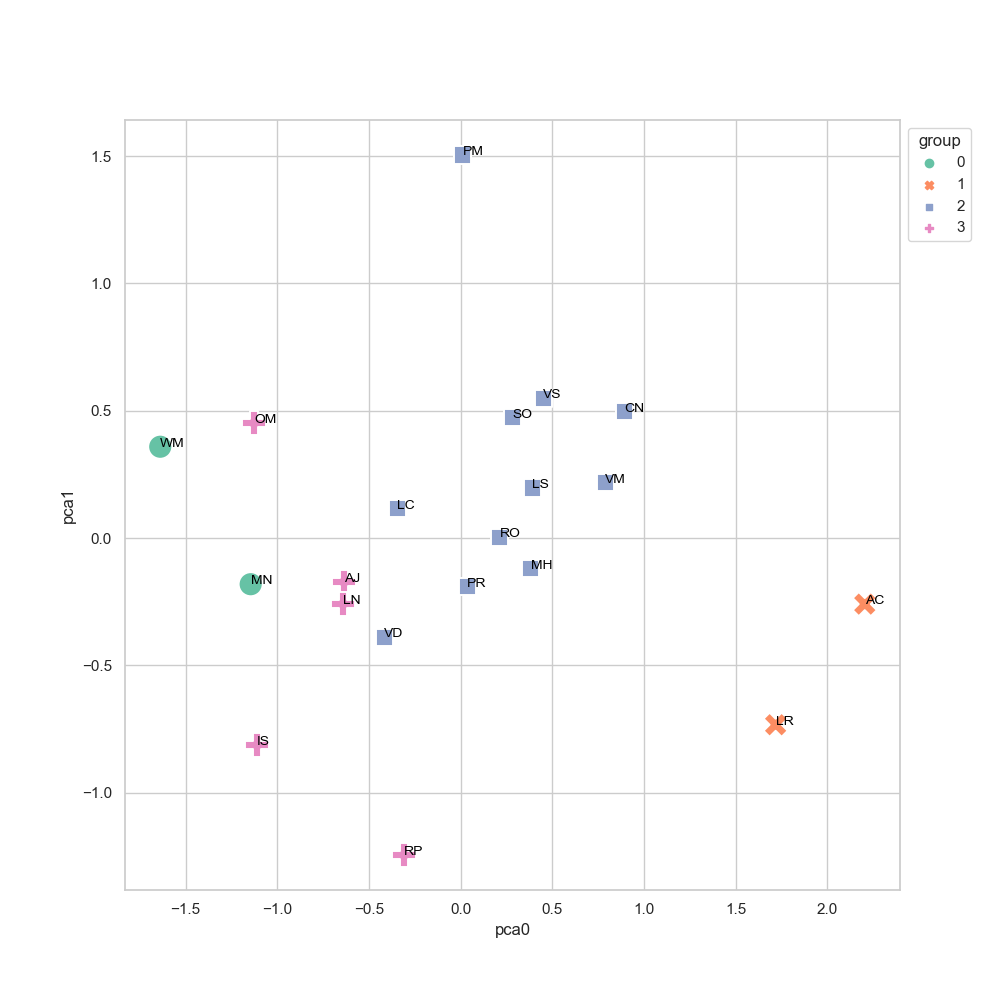
\includegraphics[width=1\linewidth]{media/clustering_4.png} 
    \caption{Caption2}
    \label{fig:clust}
\end{figure}

\section{Discussion}
\subsection{Critique des résultats vs outils / paramètres}


\subsection{Critique des résultats vs problématique}
\blindtext[3]
\section{Conclusion}
\blindtext[1]

%% Prevent urls running into margins in bibliography
\setcounter{biburlnumpenalty}{7000}
\setcounter{biburllcpenalty}{7000}
\setcounter{biburlucpenalty}{7000}

%% Add bibliography
\printbibliography[heading=bibintoc,title=References]

\end{document}

